\chapter{Sectional Curvature}\label{chap6:chap6}

Let\pageoriginale $(M,g)$ be an r.m.\@ of dimension $d$ greater than
one, and let $x$ and $y$ be two linearly independent tangent vectors
at a point $m$ of $M$. {\em Let us denote the subspace generated by
  $x$ and $y$ by $P(x,y)$.} Let $e_{1}$ and $e_{2}$ be an orthonormal
basis of $P(x,y)$. We recall that the norm on
${\displaystyle{\mathop{\wedge}^{2}}}T_{m}(M)$ is given by
$$
||x\wedge y||^{2}=||x||^{2}\cdot ||y||^{2}-(g(x,y))^{2}.
$$
Now we shall prove the following proposition.

\subsection{}\label{chap6:6.1.1}

\begin{prop*}
For $(x,y)\in T(M){\displaystyle{\mathop{\times}_{M}}}T(M)$, such that
$x$ and $y$ are linearly independent {\em the quantity}
\begin{equation*}
A(x,y)=-\dfrac{g(R(x,y)x,y)}{||x\wedge y||^{2}},\tag{6.1.2}\label{chap6:6.1.2}
\end{equation*}
depends only on $P(x,y)$.
\end{prop*}

\begin{proof}
Let $x'$ and $y'$ be two vectors such that
$$
P(x,y)=P(x',y').
$$
Then we have numbers $a$, $b$, $a'$, $b'$ such that
$$
x'=ax+by\quad\text{and}\quad y'=a'x+b'y.
$$
Then
$$
R(x',y')=R(ax+by, a'x+b'y)=(ab'-ba')R(x,y),\text{ \ by (\ref{chap2:2.5.2}) (C.R.1)}.
$$
Hence 
\begin{align*}
& g(R(x',y')x',y')=(ab'-ba')g(R(x,y)x',y')\\
& =(ab'-ba')g(R(x',y')x,y)\text{ \ by \ (\ref{chap5:5.5.5C.T.4})(C.T.4)}\\
&= (ab'-ba')^{2}g(R(x,y)x,y)
\end{align*}\pageoriginale
and further
$$
x' \wedge y'=(ab'-a'b)(x \wedge y)
$$
and hence
$$
||x' \wedge y'||^{2}=(ab'-ba')^{2}\cdot ||x \wedge y||^{2}.
$$
\end{proof}

\setcounter{subsection}{2}
\subsection{}\label{chap6:6.1.3}
For any two dimensional subspace $P$ of the tangent space $T_{m}(M)$
{\em we denote the above quantity by}
$$
A(P)=A(x,y)
$$
and call the ``function'' A {\em the sectional curvature} of $(M,g)$.

\subsection{}\label{chap6:6.1.4}
We set
\begin{align*}
\mathscr{P}(M) &= \{P\subset T_{m}(M)|m\in M\text{ \  and \ } \dim
P=2\}\\
A(M) &= \{A(P)|P\in\mathscr{P}(M)\}.
\end{align*}

\setcounter{subsection}{4}

\subsection{}\label{chap6:6.1.5}

\begin{prop*}
Let
$$
\lambda:(M,g)\to (N,h)
$$
be an isometry, then
$$
{}^M{A(P)}={}^NA(\lambda^{T}(P))\forall P\in\mathscr{P}(M).
$$
\end{prop*}

\begin{proof}
By (\ref{chap5:5.5.1}) the curvature is invariant under isometry and by
the definition of isometry the r.s.\@ is invariant under it. Hence the result.
\end{proof}

\setcounter{section}{1}
\section{Examples}\label{chap6:sec2}\pageoriginale

If $(M,g)$ is a surface then the tangent space at each point $m$ of
$M$ is two dimensional and hence $A$ assumes only one value on the set
of two dimensional subspaces of $T_{m}(M)$. Hence $A$ can be
considered as a function on $M$ itself. Now let us compute $A$ and
verify that it is nothing but the so-called Gaussian (or total)
curvature of our surface $(M,g)$.

Let us take a coordinate system $\{x,y\}$ which has been constructed
in (\ref{chap5:5.6.5}) and follow the notations of that proof. We use
propositions (\ref{chap2:2.8.7}) and (\ref{chap2:2.7.10}) and compute
$C$. Let
\begin{equation*}
\omega:t\to \omega_{\alpha}(t)\tag{6.2.1}\label{chap6:6.2.1}
\end{equation*}
be the parallel lift of $f_{\alpha}$ such that
\begin{equation*}
\omega_{\alpha}(0)=\uub{Q}(0,\alpha).\tag{6.2.2}\label{chap6:6.2.2}
\end{equation*}
Then by (\ref{chap5:5.4.9}) we have
$$
g(\omega_{\alpha}(t), \omega_{\alpha}(t))=1.
$$
Since $f'_{\alpha}(t)$ is a parallel life of $f_{\alpha}$ by
(\ref{chap5:5.4.9}) we have
$$
g(\omega_{\alpha}(t),f'_{\alpha}(t))=g(\omega_{\alpha}(0),f'_{\alpha}(0))=g(\uub{Q},\uub{P})(0,\alpha)=0. 
$$
Therefore
$$
\uub{Q}(t,\alpha)=\theta(t,\alpha)\omega_{\alpha}(t)
$$
and hence
\begin{equation*}
\widehat{\uub{Q}}(t,\alpha)=\theta(t,\alpha)\omega_{\alpha}(0). \text{ 
  \ (see \eqref{chap2:2.7.9}).}\tag{6.2.3}\label{chap6:6.2.3} 
\end{equation*}
But\pageoriginale
$$
g(\widehat{\uub{Q}}(t,\alpha),\widehat{\uub{Q}}(t,\alpha))=g(\uub{Q}(t,\alpha),\uub{Q}(t,\alpha))=k(t,\alpha)
$$
and hence by \eqref{chap6:6.2.3}
\begin{equation*}
\theta(t,\alpha)=(k(t,\alpha))^{1/2}.\tag{6.2.4}\label{chap6:6.2.4}
\end{equation*}
Now by (\ref{chap2:2.8.7})
\begin{equation*}
R(\uub{P},\uub{Q})\uub{P}=D_{P}D_{P}\uub{Q}=\frac{\partial^{2}\theta(t,\alpha)}{\partial 
  t^{2}}\cdot \omega_{\alpha}(t).\tag{6.2.5}\label{chap6:6.2.5}
\end{equation*}
We have
$$
g(R(\uub{P},\uub{Q})\uub{P},\uub{Q}) =
g\left(\frac{\partial^{2}\theta(t,\alpha)}{\partial 
  t^{2}}\omega_{\alpha}(t),
\theta(t,\alpha)\omega_{\alpha}(t)\right) =
\theta(t,\alpha)\frac{\partial^{2} \theta(t,\alpha)}{\partial t^{2}}  
$$
Further
$$
||\uub{P}\wedge\uub{Q}||^{2}=\theta(t,\alpha)^{2}.
$$
Hence by the definition of $A$ we have
\begin{equation*}
A(t,\alpha)=-\frac{t}{\theta(t,\alpha)}
\frac{\partial^{2}\theta(t,\;)}{\partial
  t^{2}}.\tag{6.2.6}\label{chap6:6.2.6} 
\end{equation*}

\setcounter{subsection}{6}
\subsection{}\label{chap6:6.2.7}
This is nothing but the value of the Gaussian curvature when computed
in a local coordinate system of the type of (\ref{chap5:5.6.5}) (see,
for example \cite{31}: formula $(3,2)$ on p.196).

\subsection{}\label{chap6:6.2.8}
The concept of sectional curvature is very powerful. Very simple
restrictions on $C$ can have deep implications. For example:

\setcounter{subsection}{8}

\subsection{}\label{chap6:6.2.9}

\begin{prop*}
If $A(M)\subset ]-\infty,0]$ then for every $m$ of $M$, $\exp_{m}$ is
    of maximal rank on $T_{m}(M)\cap \Omega$.
\end{prop*}

\begin{proof}
To prove this we use (\ref{chap2:2.8.32}). Let \pageoriginale $x\in
T_{m}(M)\cap \Omega$ and let $f:t\to \exp(t\cdot x)$ be a geodesic,
and let $h$ be a Jacobi field along $f$ such that
\begin{equation*}
h(0)=0\quad\text{and}\quad h\not\equiv 0.\tag{6.2.10}\label{chap6:6.2.10}
\end{equation*}
Then we have by (\ref{chap5:5.6.19}) ii)
\begin{align*}
\frac{d^{2}(E\circ h)}{\dt^{2}} &= 2E\circ
D_{P}h+2g(R(f',h)f',h)\geq\ldots\tag{6.2.11}\label{chap6:6.2.11}\\
&\ldots\geq 2g(R(f',h)f',h)=-A(f',h)||f'\wedge h||^{2}\geq 0.
\end{align*}
Hence the function $E\circ h$ is a non-negative convex function which
is not identically zero and hence it can vanish at most at one
point. Hence $h$ cannot vanish outside $0$ and we are through by
(\ref{chap2:2.8.32}).
\end{proof}

\setcounter{subsection}{11}
\subsection{}\label{chap6:6.2.12}
By \ref{chap2:2.5.4} $R=0$ for $(\mathbb{R}^{d},\epsilon)$. Hence
$A(\mathbb{R}^{d})=\{0\}$. 

\subsection{}\label{chap6:6.2.13}
Now let us consider the sectional curvature of the three symmetric
pairs $(\mathbb{S}^{d},\can)$, $(P^{d}(\mathbb{R}),\can)$,
$(\mathbb{R}^{d},\hyp)$ (see (\ref{chap3:sec4})). We write any of them
$M=G/H$; since $G$ operates transitively and by isometries on $M$, 
(\ref{chap6:6.1.5}) yields
\begin{equation*}
A(M)=A(T_{m_{0}}(M))\forall m_{0}\in M.\tag{6.2.14}\label{chap6:6.2.14}
\end{equation*}
By (\ref{chap3:3.4.17}) and (\ref{chap3:3.4.21}) we have in fact: $A(M)$
consists of a single real number, say $k$.

\setcounter{subsection}{14}

\subsection{}\label{chap6:6.2.15}

\begin{defi*}
An r.m.\@ $(M,g)$ for which $\exists\, k\in\mathbb{R}$ with
$A(M)=\{k\}$ is called an r.m.\@ of {\em constant sectional
  curvature.}
\end{defi*}

Hence the three symmetric pairs are of constant sectional curvature
and so is $(\mathbb{R}^{d},\can)$. The corresponding constant is $0$
for $(\mathbb{R}^{d},\can)$, $1$ for $(\mathbb{S}^{d},\can)$ or
$(P^{d}(\mathbb{R}),\can)$ by (\ref{chap6:6.3.12}) and (\ref{chap3:rems3.4.19})
$\underbar{B}$. We shall ********** move that the
constant \pageoriginale is $<0$ for
$({\overset{\bigdot}{\mathbb{R}}}{}^{d},\hyp)$. We do this by global
arguments and use the results of Chapters VII and VIII. First
$(\mathbb{R}^{d},\hyp)$ is {\em complete} in the sense of
(\ref{chap6:sec4}) because geodesics through $m_{0}$ are defined on the
whole $\mathbb{R}^{d}$ (see \ref{chap3:3.4.21} to \ref{chap3:3.4.22}). Now
this remark together with the fact that the sectional curvature is
constant and is equal to $k$ and (\ref{chap8:8.3.7}) enables us to exclude
the case $k>0$; and we are left to throw out the case $k=0$. If $k=0$
then $(\mathbb{R}^{d},\hyp)$ would be locally isometric to
$(\mathbb{R}^{d},\can)$ by (\ref{chap6:6.4.35}). By (\ref{chap5:5.1.8}) the
$\tau(\exp X)$ for $X\in \underbar{M}$ in the symmetric space
$(\mathbb{R}^{d},\hyp)$ are products of symmetries around points of
$M$; those symmetries are determined by the r.s.\@ of $(M,g)$ hence
those symmetries are the same (locally) as in
$(\mathbb{R}^{d},\can)$. In conclusion the $\tau(\exp X)$ are
isomorphic to those in $(\mathbb{R}^{d},\can)$; but the latter are the
translations and hence commute. That would imply
$[\underbar{M},\underbar{M}]=0$; it is easy to check that for
$(S0_{0}(d,1),S0(d))$ this is {\em not} the case. By using
(\ref{chap6:6.3.12}) {\em we normalise $k$ in $(\mathbb{R}^{d},\hyp)$} so as
to have $A(\mathbb{R}^{d},\hyp)=\{-1\}$.

\subsection{}\label{chap6:6.2.16}

\begin{prop*}
For any $k\in\mathbb{R}$ there exists a simply connected r.m.\@
$(M,g)$ such that $A(M,g)=\{k\}$. We may take
\begin{alignat*}{2}
& (\mathbb{S}^{d}, k^{-1/2}\cdot \can) &\text{ \ for \ } k>0\\
& (\mathbb{R}^{d},\can) & \text{ \ for \ } k=0\\
& (\mathbb{R}^{d},(-k)^{-1/2}\cdot \hyp) &\text{ \ for \ } k<0.
\end{alignat*}
\end{prop*}

\section{Geometric interpretation}\pageoriginale

\subsection{}\label{chap6:6.3.1}

\begin{defi*}
For $P\in\mathscr{P}(M)$ set
$$
\underbar{S}(P,r)=\left\{x\in P \,\big|\, ||x||=r\right\}
$$
and when $\underbar{S}(P,r)\subset\Omega$ set:
$$
S(P,r)=\exp(\underbar{S}(P,r)).
$$
{\em We call $S(P,r)$ the circle of radius $r$ in $P$.}
\end{defi*}

\subsection{}\label{chap6:6.3.2}

\begin{note*}
Let us note that if $P$ is a subspace of $T_{m}(M)$ and $\exp_{m}$ is
$r'$-O.K.\@ where $r<r'$, then the image of the circle
$\underbar{S}(P,r)$ is a compact submanifold of $M$ of dimension
one. So for $r$ sufficiently small by \ref{chap3:3.5.3} we can consider
the length $(\lg(S(P,r)))$. To compute $\lg(S(P,r))$ let us take an
orthonormal basis $\{x,y\}$ of $P$ and the parametric representation
\begin{equation*}
v:[0,2\pi]\ni \alpha\to
\text{r.e.}(\alpha)\in\underbar{S}(P,r)\tag{6.3.3}\label{chap6:6.3.3} 
\end{equation*}
where
$$
e(\alpha)=\cos\alpha\cdot x+\sin\alpha\cdot y.
$$
Now let us set
\begin{equation*}
S=\exp \circ v.\tag{6.3.4}\label{chap6:6.3.4}
\end{equation*}
Then we have
\begin{equation*}
\lg(S(P,r))=\int\limits^{2\pi}_{0}||S'||d\alpha.\tag{6.3.5}\label{chap6:6.3.5}
\end{equation*}
We have 
$$
S'=\exp^{T}\circ v'
$$
and by the definition of $v$
$$
\zeta(v'(\alpha))=\text{r.e.}\left(\alpha+\frac{\pi}{2}\right)
$$
and hence
\begin{equation*}
S'=\exp^{T}\left(\zeta^{-1}_{\text{r.e}(\alpha)}\left(\text{r.e.}\left(\alpha+
\frac{\pi}{2}\right)\right)\right).\tag{6.3.6}\label{chap6:6.3.6}    
\end{equation*}
\end{note*}

\setcounter{subsection}{6}
\subsection{}\label{chap6:6.3.7}\pageoriginale
Now if we denote by $h_{\alpha}$ the Jacobi field along
$\gamma_{e(\alpha)}$ such that
$$
h_{\alpha}(0)=0\quad\text{and}\quad
(D_{P}h_{\alpha})(0)=e\left(\alpha+\frac{\pi}{2}\right), 
$$
then by (\ref{chap5:5.6.23}) and by \eqref{chap6:6.3.6} we have
$$
S'(\alpha)=h_{\alpha}(r).
$$
Then by (\ref{chap5:5.6.19}) iii) we have
\begin{align*}
||S'(\alpha)|| &=
r+\frac{r^{3}}{6}g(R(e(\alpha),e(\alpha+\frac{\pi}{2}))e(\alpha),e(\alpha+\frac{\pi}{2}))+0(r^{3})=\tag{6.3.8}\label{chap6:6.3.8}\\
&= r-\frac{r^{3}}{6}A(P)+0(r^{3}).
\end{align*}
Hence by \eqref{chap6:6.3.5} we have
\begin{equation*}
\lg(S(P,r))=2\pi r-\frac{\pi r^{3}}{3}A(P)+0(r^{3}).\tag{6.3.9}\label{chap6:6.3.9}
\end{equation*}
Therefore we get
\begin{equation*}
A(P)=\lim\limits_{r\to 0}\frac{3}{\pi r^{3}}(2\pi
r-\lg(S(P,r))).\tag{6.3.10}\label{chap6:6.3.10} 
\end{equation*}

\setcounter{subsection}{10}

\subsection{}\label{chap6:appli6.3.11}

\begin{application*}
As an application of the above formula we note the following: Let
$(M,g)$ be an r.m.\@ and let us denote the $A$ of the manifold
$(M,kg)$ where $k>d$ by $A'$. Then we have by (\ref{chap3:3.5.4}) and
\eqref{chap6:6.3.10}.
\begin{equation*}
A'(P)=\frac{1}{k^{2}}A(P).\tag{6.3.12}\label{chap6:6.3.12}
\end{equation*}
\end{application*}

\subsection{}\label{chap6:6.3.13}

\begin{example*}
Now let us calculate $A$ for $(\mathbb{S}^{d},\can)$. We have
$$
\exp(S(\alpha))=\cos r\cdot e_{d+1}+\sin\text{ r.e}(\alpha)
$$
by the proof of (\ref{chap4:4.5.12}) and hence
$$
||S'||=\sin r.
$$
Therefore\pageoriginale
\begin{align*}
\lg(S(P,r)) &= 2\pi \sin r\\
            &= 2\pi\left(r-\frac{r^{3}}{6}+0(r^{3})\right)
\end{align*}
and hence $A(P)=1\forall P$. Instead of proceeding with circles we can
proceed, in a similar manner, with discs $\underbar{B}(m,r)\cap P$
(for some $P\in\mathscr{P}(M)$) and thus get
\begin{equation*}
A(P)=\lim\limits_{r\to 0}\frac{12}{\pi r^{4}}(\pi
r^{2}-\text{ar}(\exp\underbar{B}(m,r)\cap P)).\tag{6.3.15}\label{chap6:6.3.15}
\end{equation*}
The proof is left to the reader as an exercise.
\end{example*}

\section{A criterion for local isometry}\label{chap6:sec4}

In this article we give a result of Elie Cartan which gives a
criterion for local isometry.

To start with we shall prove a result which is purely algebraic and
asserts, essentially, that the sectional curvature determines the
curvature tensor.


\subsection{}\label{chap6:6.4.1}

\begin{prop*}
Let $V$ and $V'$ be vector spaces with euclidean structures $g$ and
$g'$, and let
$$
v:V\to V'
$$
be a euclidean isomorphism. Let $R$ and $R'$ be bilinear maps
\begin{align*}
& R:V\times V\to \End(V)\\
& R':V'\times V'\to \End(V')
\end{align*}
such that properties C.T.1, C.T.2, C.T.3 (and hence C.T.4) hold for
$R$ and $R'$. Let $A$ and $A'$ be the maps defined by means of $R$ and
$R'$ as in \eqref{chap6:6.1.2}. Then\pageoriginale
\begin{itemize}
\item[\rm i)] if an element $x$ in $V$ is such that for every $y$
  which is not linearly dependent on $x$ we have
\begin{equation*}
A(x,y)=A'(v(x),v(y))\tag{6.4.2}\label{chap6:6.4.2a}
\end{equation*}
then 
$$
R'(v(x),v(y))v(x)=v(R(x,y)x)\quad \forall y\in V.
$$
and

\item[\rm ii)] if $A'(v(x),v(y))=A(x,y)$ for every $x$ and $y$ in $V$
  which are linearly independent then
$$
R'(v(x),v(y))v(x)=v(R(x,y)z)\quad\forall x,y,z\in V.
$$
\end{itemize}
\end{prop*}

\begin{proof}
\begin{itemize}
\item[i)] Let $y$ and $z$ be elements in $V$ such that the pairs
  $\{x,y\}$, $\{x,y\}$ and $\{x,y+z\}$ are linearly independent. Then
  by hypothesis we have
\begin{equation*}
A(x,y+z)=A'(v(x),v(y+z))-=A'(v(x),v(y)+v(z)).\tag{6.4.2}\label{chap6:6.4.2}
\end{equation*}
Hence using trilinearity of $R$ and C.T.4 we have by definition of $A$
and $A'$
\begin{gather*}
\frac{A(x,y)+A(x,z)-2g(R(x,y)x,z)}{||x\wedge(y+z)||^{2}}=\ldots\tag{6.4.3}\label{chap6:6.4.3}\\
\ldots=\frac{A'(v(x),v(y))+A'(v(x),v(z))-2g(R(v(x),v(y))v(x),v(x)).}{||v(x)\wedge
  (v(y)+v(z))||^{2}} 
\end{gather*}
By \eqref{chap6:6.1.2} and the fact that $V$ is a euclidean isomorphism and
\eqref{chap6:6.4.3} we have
\begin{equation*}
g(R(x,y)x,z)=g'(R'(v(x),v(y))v(x),v(z)).\tag{6.4.4}\label{chap6:6.4.4}
\end{equation*}
Again since $v$ is a euclidean isomorphism we have
$$
g(R(x,y)x,z)=g(v^{-1}(R(v(x),v(y))v(x)),z)
$$
and,\pageoriginale since $g$ is non-degenerate, varying $z$, we have
\begin{equation*}
v(R(x,y)x)=R'(v,(x),v(y))v(x).\tag{6.4.5}\label{chap6:6.4.5}
\end{equation*}
The proof is trivial in case $x$ and $y$ are linearly dependent
(C.T.1).

\item[ii)] Substituting $x+z$ for $x$ in \eqref{chap6:6.4.5} and using
  \eqref{chap6:6.4.5} we have
$$
v(R(x,y)z)+v(R(z,y)x)=R'(v(x),v(y))v(z)+R'(v(z),v(y))v(x).
$$
i.e.
\begin{equation*}
v(R(x,y)z)-R'(v(x),v(y))v(z)=-v(R(z,y)x)-R'(v(z),v(y))v(x).\tag{6.4.6}\label{chap6:6.4.6} 
\end{equation*}
This means that if we denote the map
$$
(x,y,z)\to v(R(x,y)z)-R'(v(x),v(y))v(z)
$$
by $\theta$ we have
\begin{equation*}
\theta (x,y,z)=-\theta(z,y,x).\tag{6.4.7}\label{chap6:6.4.7}
\end{equation*}
But by C.T.1 we also have
\begin{equation*}
\theta(x,y,z)=-\theta(y,x,z).\tag{6.4.8}\label{chap6:6.4.8}
\end{equation*}
Now by \eqref{chap6:6.4.7} and \eqref{chap6:6.4.8} we have
\begin{equation*}
\theta(x,y,z)=-\theta(z,y,x)=\theta(y,z,x)\tag{6.4.9}\label{chap6:6.4.9}
\end{equation*}
i.e.\@ a cyclic permutation of $x$, $y$, $z$ does not alter
$\theta$. Hence we have
$$
3\theta(x,y,z)=\theta(x,y,z)+\theta(y,z,x)+\theta(z,x,y).
$$
But by using C.T.2.\@ we have
$$
\theta(x,y,z)+\theta(y,z,x)+\theta(z,x,y)=0.
$$
Hence
$$
\theta(x,y,z)=0.
$$
\end{itemize}
\end{proof}

\begin{example*}
As \pageoriginale an example let us note that if $A(M)=\{0\}$ then
$R=0$. 
\end{example*}

\setcounter{subsection}{9}
\subsection{}\label{chap6:6.4.10}
In what follows, if $x\in U(M)$, we denote the parallel transport
along the geodesic
$$
\gamma_{x}:t\to \exp tx
$$
from $\gamma_{x}(0)$ to $\gamma_{x}(t)$ by $\tau(x,t)$.

Then the main theorem can be stated as follows:

\setcounter{subsection}{10}

\subsection{}\label{chap6:6.4.11}

\begin{theorem*}
Let $(M,g)$ and $(N,h)$ be two r.m.'s. Let $m$ and $n$ be points in
$M$ and $N$ such that there exists
\begin{itemize}
\item[\rm i)] a euclidean isomorphism $u$ between $(T_{m}(M),g_{m})$
  and $(T_{n}(N),g_{n})$ and

\item[\rm ii)] an $r>0$ such that $\exp_{m}$ is $r$-O.K.\@ and
  $\underbar{B}(n,r)\subset{}^{N}\Omega$ and further that for every
  $x$, $y$ in $U_{m}(M)$ which are linearly in dependent and every $t$
  in $]0$, $r[$ we have
\begin{equation*}
{}^{N}C(\tau(u(x),t)u(x),\tau(u(x),t)u(y))={}^{M}C(\tau(x,t)x,\tau(x,t)y).\tag{6.4.12}\label{chap6:6.4.12} 
\end{equation*}
Then there exists $\lambda \in D(B(m,r),B(n,r))$ such that
$$
\lambda^{\ast}(h)|B(n,r)=g|(B(m,r)).
$$
\end{itemize}
\end{theorem*}

\begin{proof}
First let us prove a lemma.
\end{proof}

\setcounter{subsection}{12}

\subsection{}\label{chap6:6.4.13}

\begin{lemma*}
Under the assumptions of the above theorem, if $x\in U_{m}(M)$ and $h$
and $h_{1}$ are Jacobi fields along $\gamma_{x}$ and $\gamma_{u(x)}$
respectively such that
\begin{equation*}
h_{1}(0)=u(h(0))\quad\text{and}\quad
(D_{P}h_{1})(0)=u((D_{P}h)(0))\tag{6.4.14}\label{chap6:6.4.14} 
\end{equation*}
then
$$
h_{1}(t)=(\tau(u(x),t)\circ u\circ \tau(x,t)^{-1})h(t).
$$
\end{lemma*}

\begin{proof}
With \pageoriginale the notations \eqref{chap2:2.7.9} and \eqref{chap2:2.8.16}, by
the definition of $\tau(x,t)$ we have
\begin{equation*}
\frac{d^{2}\widehat{h}}{\dt^{2}}={}^{\widehat{M}}R(t)\widehat{h}(t)=\tau(x,t)^{-1}({}^{M}R(\gamma'_{x}(t),\widehat{h}(t)\gamma'_{x}(t)).\tag{6.4.15}\label{chap6:6.4.15} 
\end{equation*}
Since $\gamma'_{x}(t)$ is a parallel lift of $\gamma_{x}(t)$ and
$\tau(x,t)$ is the parallel transport along $\gamma_{x}$ we have
\begin{equation*}
\gamma'_{x}(t)=\tau(x,t)\gamma'_{x}(0)=\tau(x,t)x.\tag{6.4.16}\label{chap6:6.4.16}
\end{equation*}
Hence, by \eqref{chap6:6.4.15} we have
\begin{equation*}
\frac{d^{2}\widehat{h}}{\dt^{2}}=\tau(x,t)^{-1}({}^{M}R(\tau(x,t)x,\tau(x,t)\widehat{h}(t))(\tau(x,t)x)).\tag{6.4.17}\label{chap6:6.4.17} 
\end{equation*}
Let us note that the map
\begin{equation*}
v_{t}=\tau(u(x),t)\circ u\circ \tau(x,t)^{-1}\tag{6.4.18}\label{chap6:6.4.18}
\end{equation*}
From $T_{\exp tx}(M)$ to $T_{\exp t\cdot u(x)}(N)$ is a euclidean
isomorphism since parallel transport preserves the euclidean structure
(see (\ref{chap5:5.4.9})) and since $u$ is a euclidean isomorphism.

Now applying the first part of (\ref{chap6:6.4.1}) to $v$ we have
\begin{equation*}
\begin{split}
&
  {}^{N}R(\tau(u(x),t)u(x),\tau(u(x),t)u(\widehat{h}(t)))(\tau(u(x),t))u(x))=\ldots\\
&\qquad
  =v_{t}\left[{}^{M}R(\tau(x,t)x,\tau(x,t)\widehat{h}(t))(\tau(x,t)x))\right]. 
\end{split}\tag{6.4.19}\label{chap6:6.4.19}
\end{equation*}
Hence since $u$ is linear we have
\begin{gather*}
\frac{d^{2}(u\circ \widehat{h})}{\dt^{2}}=u\circ
\frac{d^{2}h}{\dt^{2}}=\ldots\\
\ldots=\tau(u(x),t)^{-1}{}^{N}R(\tau(u(x),t)u(x),\tau(u(x),t)u(\widehat{h}(t))\tau(u(x),t)u(x).\tag{6.4.20}\label{chap6:6.4.20}
\end{gather*}
Now\pageoriginale let us note, as above \eqref{chap6:6.4.16}, that
$$
\gamma'_{u(x)}(t)=\tau(u(x),t)u(x)
$$
and hence by \eqref{chap6:6.4.20}
\begin{equation*}
\frac{d^{2}(u\circ
  \widehat{h})}{\dt^{2}}={}^{\widehat{N}}R(t)((u\circ\widehat{h})(t)).\tag{6.4.21}\label{chap6:6.4.21} 
\end{equation*}
But by \eqref{chap2:2.8.4} we have
\begin{equation*}
\frac{d^{2}\widehat{h}_{1}}{\dt^{2}}={}^{\widehat{N}}R(t)\widehat{h}_{1}(t).\tag{6.4.22}\label{chap6:6.4.22} 
\end{equation*}
Hence $u\circ\widehat{h}$ and $\widehat{h}_{1}$ satisfy the same
second order differential equation; and further the assumptions
\eqref{chap6:6.4.14} are the same as
$$
\widehat{h}_{1}(0)=(u\circ\widehat{h})(0)\text{ and }
\frac{d\widehat{h}_{t}}{\dt}(0)=u\left(\frac{d\widehat{h}}{\dt}(0)\right)=\frac{d(u\circ\widehat{h})}{\dt}(0) 
$$
since $u$ is linear and this means that $\widehat{h}_{1}$ and
$u\circ\widehat{h}$ satisfy the same differential equation with the
same initial conditions. Hence
\begin{equation*}
\widehat{h}_{1}=u\circ \widehat{h}\tag{6.4.23}\label{chap6:6.4.23}
\end{equation*}
and hence
\begin{equation*}
h_{1}(t)=v_{t}\circ h(t) \;\forall t.\tag{6.4.24}\label{chap6:6.4.24}
\end{equation*}
\end{proof}

\noindent
{\bf Proof of the theorem.}~By (\ref{chap4:4.2.6}) we have to define
$\lambda$ by:
\begin{equation*}
\lambda={}^{N}\exp_{n}\circ u\circ
({}^{M}\exp_{m}|\underbar{B}(m,r))^{-1};\tag{6.4.25}\label{chap6:6.4.25} 
\end{equation*}
we check that $\lambda$ is indeed a local isometry. To show this we
have only \pageoriginale to prove that the map
$$
\lambda^{T}_{a}:T_{a}(M)\to T_{\lambda(a)}(N)
$$
is a euclidean isomorphism $\forall a\in B(m,r)$. We first note, since
$u$ is linear, that
\begin{equation*}
u^{T}\circ \zeta^{-1}_{x}=\zeta^{-1}_{u(x)}\circ u, x\in
T_{m}(M).\tag{6.4.26}\label{chap6:6.4.26} 
\end{equation*}
Now, for $a=m$, using (\ref{chap1:1.4.6}) we have
$$
\lambda^{T}_{m}=\zeta_{0_{n}}\circ u^{T}\circ
\zeta^{-1}_{0_{m}}=\zeta_{0_{n}}\circ \zeta^{-1}_{0_{n}}\circ u=u
$$
and hence we are through in case $a=m$. In the other case $\exists\,
t\in ]0$, $r[$ and $x\in U_{m}(M)$ such that
\begin{equation*}
a={}^{M}\exp_{m}(t\cdot x).\tag{6.4.27}\label{chap6:6.4.27}
\end{equation*}
Now let $z$ be any element of $T_{a}(M)$. Since ${}^{M}\exp_{m}$ is
$r$-O.K. and $a\in B(m,r)$ there exists an $\omega$ in $T_{t\cdot
  x}(T_{m}(M))$ such that
\begin{equation*}
z={}^{M}\exp^{T}_{m}(\omega).\tag{6.4.28}\label{chap6:6.4.28}
\end{equation*}
Now set
\begin{equation*}
y=\zeta(\omega).\tag{6.4.29}\label{chap6:6.4.29}
\end{equation*}
By (\ref{chap5:5.6.23}) we have
\begin{equation*}
z=h(||t\cdot x||)=h(t)\tag{6.4.30}\label{chap6:6.4.30}
\end{equation*}
where $h$ is the Jacobi field along $\gamma_{x}$ such that
\begin{equation*}
h(0)=0\quad\text{and}\quad D_{P}h(0)=\frac{y}{||t\cdot
  x||}=\frac{y}{t}.\tag{6.4.31}\label{chap6:6.4.31} 
\end{equation*}
Further by the definition of $\lambda$ and $y$ we have
\begin{equation*}
\lambda^{T}(z)=({}^{N}\exp_{n})^{T}\circ
u^{T}\circ(\zeta^{-1}_{tx}(y))=({}^{N}\exp_{n})^{T}\circ
\zeta^{-1}_{tx}(u(y))\quad\text{by \eqref{chap6:6.4.25}}\tag{6.4.32}\label{chap6:6.4.32}
\end{equation*}
and \pageoriginale hence, again by (\ref{chap5:5.6.23}), we have
\begin{equation*}
\lambda^{T}(z)=h_{1}(||t\cdot u(x)||)=h_{1}(t)\tag{6.4.33}\label{chap6:6.4.33}
\end{equation*}
(since $u$ is a euclidean isomorphism) where $h_{1}$ is the Jacobi
field along $\lambda_{u(x)}$ with
\begin{equation*}
h_{1}(0)=0\quad\text{and}\quad D_{P}h_{1}(0)=\frac{u(y)}{||t\cdot
  u(x)||}=\frac{u(y)}{t}=u\left(\frac{y}{t}\right).\tag{6.4.34}\label{chap6:6.4.34} 
\end{equation*}
Now considering $v_{t}$, $h$, $h_{1}$ and applying (because of
\eqref{chap6:6.4.31} and\break \eqref{chap6:6.4.34}) the lemma we have
\begin{equation*}
h_{1}(t)=v_{t}\circ h(t) \; \forall t\tag{6.4.35}\label{chap6:6.4.35}
\end{equation*}
where $v_{t}$ is given by \eqref{chap6:6.4.18}. But $v_{t}$ is a euclidean
isomorphism and hence the result follows by \eqref{chap6:6.4.33},
\eqref{chap6:6.4.33} and (\ref{chap6:6.4.36}).

\setcounter{subsection}{34}

\subsection{}\label{chap6:s6.4.35}

\begin{coro*}
Any two r.m.'s of constant sectional curvature $k$ are locally
isometric. Hence, by \eqref{chap6:6.3.12} any r.m.\@ of constant sectional
curvature $k$ is locally isometric to
\begin{align*}
&(\mathbb{S}^{d},k^{-1/2},\can)\text{ \ if \ } k>0\\
& (\mathbb{R}^{d},\epsilon)\text{ \ if \ } k=0\\
& (\mathbb{R}^{d},k^{-1/2},\hyp)\text{ \ if \ }k<0.
\end{align*}
\end{coro*}

\subsection{}\label{chap6:6.4.36}


\begin{remarks*}
\begin{enumerate}
\renewcommand{\labelenumi}{\theenumi)}
\item For a global result on manifolds of constant sectional curvature
  see (\ref{chap7:sec7})

\item For a global result in general see \cite{1}

\item In general the knowledge of sectional curvature (which is the
  same by (\ref{chap6:6.4.1}) as that of curvature tensor) does not
  determine, even locally, the r.s. In fact there exist r.m.'s $(M,g)$
  and $(N,h)$ such \pageoriginale that there exists a diffeomorphism
  $\lambda$ such that 
\begin{itemize}
\item[i)] ${}^{M}A(P)={}^{N}A(\lambda^{T}(P))\forall
P\in\mathscr{P}(M)$ and

\item[ii)] $\lambda$ is not an isometry. 
\end{itemize}
\end{enumerate}
\end{remarks*}

The theorem (\ref{chap6:6.4.11}) says that if for all geodesics through a
point, $\lambda$ preserves the sectional curvature of planes
corresponding under parallel transport along geodesics, then $\lambda$
is a local isometry at this point.

\section{Jacobi fields in symmetric pairs}\label{chap6:sec5}
\quad 
In this article we assume that $(M,g)$ is an r.m.\@ associated to a
symmetric pair $(G,H)$ and follow the notation of (\ref{chap3:sec3}) and of
(\ref{chap6:sec4}).

Let $f$ be a geodesic in $M$. Then by (\ref{chap5:5.1.8}) the parallel
transport $\tau(f',t)$ along $f$ is given by the tangent maps of
isometries. Hence by (\ref{chap5:5.1.6}) we have the:

\subsection{}\label{chap6:6.5.1}

\begin{prop*}
Let $m$ be a point of $(M,g)$. Then 
\begin{itemize}
\item[\rm i)]
  $\tau(x,t)(R(x,y)x)=R(\tau(x,t)x$, $\tau(x,t)y)\tau(x,t)x \; \forall
  x\in  U_{m}(M)$, $\forall y\in T_{m}(M)$ and 

\item[\rm ii)] $A(x,y)=A(\tau(x,t)x$, $\tau(x,t)y)$ if $x$, $y$ are
  linearly independent.
\end{itemize}
\end{prop*}

\subsection{}\label{chap6:rem6.5.2}%%%

\begin{remark*}
The converse of (\ref{chap6:6.5.1}) ii) is true: an r.m.\@ where
parallel transport preserves sectional curvature is locally isometric
to a symmetric space: see Chapter IV of \cite{14}. The \pageoriginale
relation (\ref{chap6:6.5.1}) i) gives a complete information about Jacobi
fields of $M$. For now the formula \eqref{chap6:6.4.15} gives
\begin{equation*}
\frac{d^{2}\widehat{h}}{\dt^{2}}=R(x,\widehat{h}(t))x.\tag{6.5.3}\label{chap6:6.5.3}
\end{equation*}
{\em Now let us introduce the endomorphism $\overline{R}(x)$ of
$T_{m}(M)$ by setting:}
\begin{equation*}
\overline{R}(x)y=R(x,y)x\quad\forall y\in T_{m}(M).\tag{6.5.4}\label{chap6:6.5.4}
\end{equation*}
Then by \eqref{chap5:5.5.5C.T.4} we have
$$
g(\overline{R}(x)y,z)=g(R(x,y)x,z)=g(R(x,z)x,y)=g(\overline{R}(x)z,y)
$$
and hence $\overline{R}(x)$ is symmetric. Now by the reduction process
of quadratic forms to diagonal form we see that there exist real
numbers $\lambda_{1},\ldots,\lambda_{d}$ and an orthonormal basis
$\{x_{1},\ldots,x_{d}\}$ of $T_{m}(M)$ such that
\begin{equation*}
\overline{R}(x)x_{i}=\lambda_{i}x_{i}, i=1,\ldots,d.\tag{6.5.5}\label{chap6:6.5.5}
\end{equation*}
But since $\overline{R}(x)x=0$, and $x$ is in $U_{m}(M)$ we can assume
that $x_{1}=x$ and $\lambda_{1}=0$. For any lift $h$ of $f$ into
$T(M)$ there correspond functions $\psi_{1},\ldots,\psi_{d}$ such that
$$
\widehat{h}(t)=\sum_{i}\psi_{i}(t)x_{i}
$$
and by (\ref{chap2:2.7.10}) we have
$$
\frac{d^{2}\widehat{h}(t)}{\dt^{2}}=\sum_{i}\frac{d^{2}\psi_{i}(t)}{\dt^{2}}\cdot
x_{i}. 
$$
Further if $h$ is a Jacobi field then by \eqref{chap6:6.5.3} we have
\begin{equation*}
\frac{d^{2}\psi_{i}}{\dt^{2}}=\lambda_{i}\psi_{i}.\tag{6.5.6}\label{chap6:6.5.6}
\end{equation*}\pageoriginale
In particular we define for $i=1,\ldots,d$ a Jacobi field $h_{i}$ by
$$
h_{i}(0)=0\quad\text{and}\quad (D_{P}h_{i})(0)=x_{i}.
$$
Then we have
\begin{equation*}
h_{i}(t)=
\begin{cases}
(-\lambda_{i})^{-1/2}\cdot\sin(\sqrt{-\lambda_{i}}\cdot t)\cdot x_{i}
  &\text{if  \ } \lambda_{i}<0\\
t\cdot x_{i} & \text{if \ } \lambda_{i}=0\\
(\lambda_{i})^{-1/2}\cdot \sh(\sqrt{\lambda_{i}}\cdot t)\cdot x_{i} &
\text{if \ } \lambda_{i}>0.
\end{cases}\tag{6.5.7}\label{chap6:6.5.7}
\end{equation*}
Let us note that by \eqref{chap5:5.5.5C.T.4}
\begin{equation*}
\lambda_{i} = g(\overline{R}(x)x_{i},x_{i}) =
g(R(x,x_{i})x,x_{i})=-A(x,x_{i}).\tag{6.5.8}\label{chap6:6.5.8}   
\end{equation*}
\end{remark*}

\section{Sectional curvature of S.C.-manifolds}\label{chap6:sec6}

In this article we assume that $(M,g)$ stands for an S.C.-manifold and
follow the notations of (\ref{chap3:sec4}). We already know (by (\ref{chap6:sec2}))
that $A(M)=\{1\}$ for $(\mathbb{S}^{d},\can)$ and
$(P^{d}(\mathbb{R}),\can)$. In the following proposition we think of
the remark (\ref{chap4:4.5.6}) for the case of $P^{2}(\Gamma)$: then
``$y$ is orthogonal to $K\cdot x$'' stands for ``$y$ is orthogonal to
the fibre through $x$''. Note that the proof below, for the case of
$P^{2}(\Gamma)$, uses only (\ref{chap4:4.5.7}).


\subsection{}\label{chap6:6.6.1}

\begin{prop*}
Let $(M,g)$ be an S.C.-manifold, which is $(P^{n}(K),\can)$ with
$n>1$, $K\neq\mathbb{R}$ or $P^{2}(\Gamma)$.

Then 
$$
A(M)=\{1,4\};
$$
more \pageoriginale precisely, if $x$, $y$ are
$\mathbb{R}$-independent:
\begin{itemize}
\item[\rm i)] $A(x,y)=4$ if $x$, $y$ are $K$-dependent

\item[\rm ii)] $A(x,y)=1$ if $y$ is orthogonal to $K\cdot x$.
\end{itemize}
\end{prop*}

\begin{proof}
***** (6.6.2). By (\ref{chap4:4.5.4}) all geodesics through $m_{0}$ are
closed and are of length $\pi$. By (\ref{chap2:2.8.26}) every Jacobi
field along a geodesic $\gamma_{x}$ can be realised as the variations
of vectors along a family of geodesic curves. Hence it follows that
any Jacobi field along a geodesic through $m_{0}$ which vanishes at
$m_{0}$ for $t=0$ vanishes again for $t=\pi$. Now let $x\in
U_{m_{0}}(M)$ and the corresponding objects
$$
\{x=x_{1},x_{2},\ldots,x_{d}\},
\{\lambda_{1}=0,\lambda_{2},\ldots,\lambda_{d}\},
\{h_{1},h_{2},\ldots,h_{d}\} 
$$ 
be as in (\ref{chap6:sec5}). Hence $h_{i}(\pi)=0$ implies, necessarily by
\eqref{chap6:6.5.7} that $\lambda_{i}<0$ and we have
\begin{equation*}
h_{i}(t)=(-\lambda_{i})^{-1/2}\cdot \sin (\sqrt{-\lambda_{i}}\cdot
t)\cdot x_{i}.\tag{6.6.3}\label{chap6:6.6.3}
\end{equation*}
Again $h_{i}(\pi)=0$ implies $\lambda_{i}\in\{-1,-4,-9,\ldots\}$. Now
by (\ref{chap2:2.8.32}) and (\ref{chap4:4.5.12}) we know $h_{i}(t)$ cannot
vanish on $]0$, $\dfrac{\pi}{2}[$, hence $\lambda_{i}=-1$ or $-4$.

This implies already that $A(M)\subset \{1,4\}$ for the eigen values
of $\overline{R}(x)$ on the orthogonal complement of $x$ are $1$ or
$4$ (by \eqref{chap6:6.5.8}).
\begin{itemize}
\item[(i)] Now let $x_{i}$ be $K$-dependent on $x$ and let $h$ be the
  Jacobi field along $\gamma_{x}$ given by the variations of vectors
  along the one parameter family of geodesics
$$
\gamma_{(\cos\alpha)\cdot x+(\sin\alpha)\cdot x_{i}}(t).
$$
Then, \pageoriginale since each $(\cos\alpha)\cdot x+(\sin\alpha)\cdot
x_{i}$ is $K$-dependent on $x$ by (\ref{chap4:4.5.7}) (ii), it follows
that all of them meet at $t=\dfrac{\pi}{2}$ and hence
$$
h_{i}\left(\frac{\pi}{2}\right)=0,
$$
hence $\lambda_{i}=-4$.

\item[(iii)] Suppose conversely that $\lambda_{i}=-4$ and set
$$
e(\alpha)=(\cos\alpha)\cdot x+(\sin \alpha)\cdot
x_{i}\quad\text{and}\quad S(\alpha)=\exp\left(\frac{\pi}{2}\cdot
e(\alpha)\right). 
$$
Then (see \eqref{chap6:6.3.6}) we have
$$
S'(\alpha)=\exp^{T}_{m_{0}}\left(\zeta^{-1}_{\frac{\pi}{2}\cdot
  e(\alpha)}\left(\frac{\pi}{2}\cdot
e\left(\alpha+\frac{\pi}{2}\right)\right)\right). 
$$
But by (\ref{chap5:5.6.23}) we have
\begin{equation*}
S'(\alpha)=h\left(\frac{\pi}{2}\right)\tag{6.6.6}\label{chap6:6.6.6}
\end{equation*}
where $h$ is the Jacobi field along $\gamma_{e(\alpha)}$ satisfying
the equations
$$
h(0)=0\quad\text{and}\quad D_{P}h(0)=e\left(\alpha+\frac{\pi}{2}\right).
$$

Since the subspaces generated by the pairs
$\{e(\alpha),e(\dfrac{\pi}{2}+\alpha)\}$ and $\{x,x_{i}\}$ are the
same we have
$$
A\left(e(\alpha),e\left(\frac{\pi}{2}+\alpha\right)\right)=A(x,x_{i})=4. 
$$
Since $4$ is the {\em maximum value} of the quadratic form
$A(e(\alpha),\ast)$, it follows that $e(\alpha+\dfrac{\pi}{2})$ is an
eigen vector of $\overline{R}(e(\alpha))$. Hence in view of
\eqref{chap6:6.6.3} we have
$$
h\left(\frac{\pi}{2}\right)=0
$$
and hence by \eqref{chap6:6.6.6} we have
$$
S'(\alpha)=0 \; \forall \alpha.
$$
Hence \pageoriginale $S(\alpha)=S(0)=\exp(\dfrac{\pi}{2}\cdot x)$ for
every $\alpha$, and hence in particular
$$
\exp\left(\frac{\pi}{2}\cdot
x_{i}\right)=S(1)=S(0)=\exp\left(\frac{\pi}{2}\cdot x\right).
$$
Then by (\ref{chap4:4.5.7}) we see that $\{x,x_{i}\}$ are
$K$-dependent. We conclude that $\lambda_{i}=-4$ if and only if
$x_{i}$ is $K$-dependent on $x$. Since $\{x_{i}\}$ is an orthogonal
basis, we see that $\lambda_{i}=-1$ if and only if $x_{i}$ is
orthogonal to $K\cdot x$. Hence $\overline{R}(x)$ is $-4$ times the
identity on the orthogonal complement of $x$ in $Kx$ and $-1$ times
the identity on the orthogonal complement of $Kx(\text{in }
T_{m_{0}})$. Thus, if $K\neq \mathbb{R}$, $\exists\, i$ such that
$\lambda_{i}=-4$; if $n>1$, then $\exists\, i$ such that $\lambda_{i}=-1$.
\end{itemize}
\end{proof}

\setcounter{subsection}{7}

\subsection{}\label{chap6:6.6.8}

\begin{remark*}
Let $(M,g)$ be any S.C.-manifold and $x\in U(M)$. Then (upto a
permutation of the $i$'s) we have for the associated set
$\{\lambda_{i}\}(i\geq 2)$
\begin{center}
\begin{tabular}{>{$}l<{$}@{\;:\;}>{$}l<{$}}
P^{d}(\mathbb{R}),\mathbb{S}^{d}(\mathbb{R}) & \lambda_{i}=-1\forall
i\\
P^{n}(\mathbb{C}) & \lambda_{2}-4, \lambda_{i}=-1\quad i\geq 3\\
P^{n}(\mathbb{H}) & \lambda_{2}=\lambda_{3}=-4,\lambda_{i}=-1\quad
i\geq 5\\
P^{2}(\Gamma) &
\lambda_{i}=-4:i=2,\ldots,8,\lambda_{i}=-1:i=9,\ldots,16. 
\end{tabular}
\end{center}
\end{remark*}

\section{Volumes of S.C.\@ manifolds}\label{chap6:sec7}

Now we give an example of calculation. We show how the exponential map
and Jacobi fields can be used to estimate the volume of an r.m. In
sharper recent results this has been systematically done to get bounds
for $\Vol(M,g)$ in terms of those of $A(M)$ (see \cite{33},
Ch. 11)). Here we shall be content with the treatment of a case where
the computation can be explicitly carried out and, at the same time,
is simple enough \pageoriginale to exhibit clearly the method
involved. The same method works in more general situations but we do
not have space here to handle them.

We compute the volume of an S.C.\@ manifold. Since we know (see
(\ref{chap3:3.5.6})) that 
$$
\Vol(\mathbb{S}^{d},\can)=2\Vol(P^{d}(\mathbb{R}),\can),
$$
we may assume that $(M,g)$ is different from $\mathbb{S}^{d}$. First
let us note that the fact that any point $m$ can be joined to $m_{0}$
by a geodesic (see proof of (\ref{chap4:4.5.4})) together with the fact
that each geodesic is of length $\pi$ implies that 
$$
\exp_{m_{0}}(\overline{\underline{B}(m_{0},\pi/2)})=M.
$$
But $\exp_{m_{0}}$ is a $C^{\infty}$-map and the set
$\overline{\underline{B}(m_{0},\pi/2)}-\underline{B}(m_{0},\pi/2)$ has
measure zero. Hence we have
\begin{align*}
\Vol(M,g) &=
\Vol(\exp_{m_{0}}(\overline{\underline{B}(m_{0},\pi/2)})\\
&= \Vol(\exp_{m_{0}}(\underline{B}(m_{0},\pi/2))\\
&= \Vol(B(m_{0},\pi/2)).
\end{align*}
By (\ref{chap4:4.5.12}) $\exp_{m_{0}}$ is $\pi/2$-O.K., and if we fix an
orientation on $T_{m_{0}}(M)$ and pass to the canonical volume form
$\sigma$ on $B(m_{0},\pi/2)$, (see (\ref{chap3:sec5}))we have
$$
\Vol(B(m_{0},\pi/2))=\int\limits_{B(m_{0},\pi/2)}\sigma=\int\limits_{\underline{B}(m_{0},\frac{\pi}{2})}(\exp_{m_{0}})^{\ast}\sigma.
$$
To \pageoriginale compute the latter we look upon
$\underline{B}(m,\pi/2)-\{0\}$ as 
diffeomorphic to the product manifold
$$
W=]0, \pi/2[\times U_{m_{0}}(M),
$$
under the map
$$
n:W\ni (t,x)\to t\cdot x\in \underline{B}(m_{0},\pi/2)-\{0\}.
$$
Here $n$ clearly is a diffeomorphism and since the point $m_{0}$ has
zero measure we have
\begin{align*}
\vol(M,g) &=
\int\limits_{\underline{B}(m_{0},\pi/2)}(\exp_{m_{0}})^{\ast}\sigma\\
          &= \int\limits_{W}(\exp_{m_{0}}\circ n)^{\ast}\sigma.
\end{align*}
Now let us introduce two projection maps on $W$ defined by the
equations
$$
p(t,x)=t\quad\text{and}\quad q(t,x)=x.
$$
Denoting the canonical volume form on $U_{m_{0}}(M)$ by $\theta$ we
get a volume form
$$
\omega=p^{\ast}(\dt)\wedge q^{\ast}(\theta)
$$
on $W$. But then there exists a function $\varphi$ such that
$$
(\exp_{m_{0}}\circ n)^{\ast}\sigma=\varphi\omega.
$$
and we will be through if we know $\varphi$.

\subsection{}\label{chap6:6.7.1}

\begin{lemma*}
With the above notation
$$
\varphi(t,x)=\left(\frac{\sin 2t}{2}\right)^{\alpha}\quad (\sin
t)^{d-\alpha-1}
$$
for every $x$ in $\mathbb{S}^{d-1}$ and $t$ in $]0$, $\pi/2[$, where
\begin{align*}
\alpha &= 0\text{ \ for \ } P^{d}(\mathbb{R});\alpha=1\text{ \ for \ }
P^{d}(\mathbb{C});\\
\alpha &= 3 \text{ \ for \ } P^{d}(\mathbb{H});\alpha = 7 \text{
  \  for \ } P^{2}(\Gamma).
\end{align*}\pageoriginale
\end{lemma*}

\begin{proof}
Let us follow the notation of article 6. The tangent space
$T_{(t,x)}\unskip\break (W)$ is in a natural way isomorphic to $T_{t}(\,]0$,
    $\pi/2[\,)\times T_{x}(U_{m_{0}}(M))$. But (see \ref{chap5:5.2.9}) the
      vectors $\{\zeta^{-1}_{x}x_{2},\ldots,\zeta^{-1}_{x}x_{d}\}$
      form a basis for $T_{x}(U_{m_{0}}(M))$ and hence
$$
\{(P,0),(0,\zeta^{-1}_{x}x_{2}),\ldots,(0,\zeta^{-1}_{x}x_{d})\}
$$
is a basis for $T_{(t,x)}(M)$ such that
$$
\omega((P,0),(0,\zeta^{-1}_{x}x_{2}),\ldots,(0,\zeta^{-1}_{x}x_{d}))=1.
$$
Hence we have
\begin{align*}
\varphi(t,x) &= ((\exp_{m_{0}}\circ
n)^{\ast})((P,0),(0,\zeta^{-1}_{x}x_{2}),\ldots,(0,\zeta^{-1}_{x}x_{d}))=\\ 
&=
(\exp^{T}_{m_{0}}(n^{T}(P,0),\exp^{T}_{m_{0}}(n^{T}(0,\zeta^{-1}_{x}x_{2}),\ldots,)\\
&\qquad\ldots,\exp^{T}_{m_{0}}(n^{T}(0,\zeta^{-1}_{x}x_{d}))). 
\end{align*}
Since the map
$$
n:(t,x)\to t\cdot x
$$
is bilinear, we have
$$
n^{T}(0,\zeta^{-1}_{x}x_{i})=t\cdot \zeta^{-1}_{t\cdot
  x}x_{i}\quad\text{and}\quad n^{T}(P,0)=\zeta^{-1}_{tx}x.
$$
Further by (\ref{chap5:5.6.32}) the images
$$
\exp^{T}_{m_{0}}(\zeta^{-1}_{tx}x_{1}),\exp^{T}_{m_{0}}(\zeta^{-1}_{tx}x_{2}),\ldots 
$$
are mutually orthogonal and
$$
||\exp^{T}_{m}(\zeta^{-1}_{tx}x)||=||\zeta^{-1}_{tx}x||=1.
$$\pageoriginale
Hence we have
$$
\varphi(t,x)=\prod_{i>2}||\exp^{T}_{m_{0}}(\zeta^{-1}_{tx}t\cdot
x_{i})||. 
$$
But by (\ref{chap5:5.6.23}) we have
$$
\exp^{T}_{m_{0}}(\zeta^{-1}_{t\cdot x}(t\cdot x_{i}))=h_{i}(||tx||)=h_{i}(t)
$$
where $h_{i}$ is the Jacobi field along $\gamma_{x}$ such that
$$
h_{i}(0)=0\quad\text{and}\quad (D_{P}h_{i})(0)=\frac{t\cdot
  x_{i}}{||t\cdot x_{i}||}=x_{i}. 
$$
But then by \eqref{chap6:6.5.7} we have
$$
h_{i}(t)=(-\lambda_{i})^{-1/2}\cdot \sin(\sqrt{-\lambda_{i}}\cdot
t)\cdot x_{i}
$$
and hence
\begin{equation*}
\varphi(t,x)=\prod_{i>2}(-\lambda_{i})^{-1/2}\cdot \sin
(\sqrt{-\lambda_{i}}\cdot t)\tag{6.7.2}\label{chap6:6.7.2}
\end{equation*}
and we are through by (\ref{chap6:6.6.8}).
\end{proof}

Now let us note that since all euclidean structures of the same
dimension are isomorphic we have
$$
\Vol(U_{m}(M),g_{m})=\Vol(\mathbb{S}^{d-1},\can) \; \forall m\in M.
$$
We set
\begin{equation*}
\Vol(\mathbb{S}^{d},\can)=\mycirc{d}.\tag{6.7.3}\label{chap6:6.7.3}
\end{equation*}
Hence by (\ref{chap0:0.3.17}):
\begin{gather*}
\int\limits_{W}\varphi(t,x)\cdot p^{\ast}(\dt)\wedge
q^{\ast}(\theta)=\int\limits_{U_{m_{0}}(M)}\left(\int\limits^{\pi/2}_{0}\varphi(t,x)\cdot
\dt\right)\cdot \theta=\\
=\left(\int\limits_{U_{m_{0}(M)}}\theta\right)\cdot\int\limits^{\pi/2}_{0}\varphi(t,x)\cdot \dt
\end{gather*}\pageoriginale
since $\varphi$ is independent of $x$.

Hence
\begin{equation*}
\Vol(M,g)=\oval{d-1}\cdot \int\limits^{\pi/2}_{0}\left(\frac{\sin
  2t}{2}\right)^{\alpha}\cdot \sin^{d-\alpha-1}t\cdot
\dt.\tag{6.7.4}\label{chap6:6.7.4} 
\end{equation*}
First \eqref{chap6:6.7.4} gives for the \mycirc{d}'s the recurrence formula:
$$
\mycirc{d}=2\cdot
\Vol(P^{d}(\mathbb{R}),\can)=2\oval{d-1}\int\limits^{\pi/2}_{0}\sin^{d-1}t\cdot
\dt.
$$
The value of $\int^{\pi/2}_{0}\sin^{d-1}t\cdot \dt$ is well
known. Using this, we get
{\fontsize{9}{11}\selectfont
\begin{gather*}
\oval{2n}=2\cdot\frac{(2\pi)^{n}}{(2n-1)\cdot (2n-3)\ldots
  3.1},\oval{2n-1}=2\cdot
\frac{\pi^{n}}{(n-1)!}\tag{6.7.5}\label{chap6:6.7.5}\\
\Vol(P^{2n}(\mathbb{R}),\can)=\frac{(2\pi)^{n}}{(2n-1)\cdot
  (2n-3)\ldots 3.1},\Vol(P^{2n-1}(\mathbb{R}),\can)=\frac{\pi^{n}}{(n-1)!}
\end{gather*}}\relax

Note, in particular, that
\begin{equation*}
\mycirc{2}=\Vol(\mathbb{S}^{2},\can)=4\pi,\Vol(P^{2}(\mathbb{R}),\can)=2\pi.\tag{6.7.6}\label{chap6:6.7.6} 
\end{equation*}
For $P^{n}(\mathbb{C})$ we compute
$$
\int\limits^{\pi/2}_{0}\frac{\sin 2t}{2}\cdot \sin^{2n-2}t\cdot
\dt=\int\limits^{\pi/2}_{0}\sin^{2n-1}t\cdot\cos t\cdot \dt=\frac{1}{2n};
$$
with \eqref{chap6:6.7.5} this gives
\begin{equation*}
\Vol(P^{n}(\mathbb{C}),\can)=\frac{\pi^{n}}{n!}\tag{6.7.7}\label{chap6:6.7.7}
\end{equation*}
By \pageoriginale the same kind of straightforward computations,
\begin{gather*}
\Vol(P^{n}(\mathbb{H}),\can)=\frac{\pi^{2n}}{(2n+1)!},\tag{6.7.8}\label{chap6:6.7.8}\\
\Vol(P^{2}(\Gamma),\can)=\frac{\pi^{8}}{11.10.9.8.7.6.5.4.}.\tag{6.7.9}\label{chap6:6.7.9} 
\end{gather*}

\setcounter{subsection}{9}

\subsection{}\label{chap6:6.7.10}

\begin{remark*}
Using \eqref{chap3:3.4.10} and (\ref{chap3:rems3.4.19}), and the formula
(\ref{chap0:0.3.17}) one would get
\begin{align*}
\Vol(P^{n}(\mathbb{C}),\can) &= \oval{2n+1}/\mycirc{1},\\
\Vol(P^{n}(\mathbb{H}),\can) &= \oval{4n+3}/\mycirc{3},
\end{align*}
which agrees with \eqref{chap6:6.7.5}, \eqref{chap6:6.7.6}, \eqref{chap6:6.7.7}.

Note also that
$$
P^{2}(\Gamma)=\mycirc{23}/\mycirc{7}.
$$
But here it is impossible to get that formula through a fibration
because one knows from algebraic topology (non existence of elements
of Hopf invariant one) that there does not exist a fibration
\[
\xymatrix{
\mathbb{S}^{23}\ar[d]^{\mathbb{S}^{7}}\\
P^{2}(\Gamma)
}
\]
Next, we give a formula which will be used later on:
\begin{equation*}
I=\int\limits_{x\in\mathbb{S}^{d}}|x\cdot x_{0}|\cdot\sigma=
\frac{2}{d}\oval{d-1},\tag{6.7.11}\label{chap6:6.7.11}
\end{equation*}
where $\sigma$ is the canonical volume form of $(\mathbb{S}^{d},\can)$
and $x_{0}$ a fixed point in $\mathbb{S}^{d}$. 
\end{remark*}

\begin{proof}
If\pageoriginale $x$ is at the distance $t$ from $x_{0}$ {\em on}
$\mathbb{S}^{d}$ then $x\cdot x_{0}=\cos t$. We make the computations
on $P^{d}(\mathbb{R})$ instead of $\mathbb{S}^{d}$ using the remark
that $x\to |x\cdot x_{0}|$ is invariant under the antipodal map of
$\mathbb{S}^{d}$. 
\begin{figure}[H]
\centering
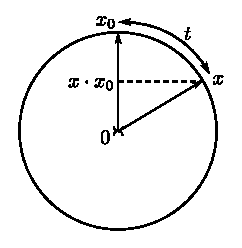
\includegraphics[scale=1.1]{figures/chap6-fig1.eps}
\end{figure}
Thus $I=2\int_{p^{d}(\mathbb{R})}p(|x\cdot
x_{0}|)\cdot\overline{\sigma}$ where $\overline{\sigma}$ denotes the
volume element on $p^{d}(\mathbb{R})$. We follow the computation of
$\Vol(P^{d}(\mathbb{R}),\can)$ as above, taking $p(x_{0})=m_{0}$. This
gives
\begin{align*}
I &=
2\int\limits_{U_{m_{0}}(M)}\left(\int\limits^{\pi/2}_{0}\varphi(t,x)\cdot
|\cos t|\cdot \dt\right)=\ldots\\
&= 2\oval{d-1}\int\limits^{\pi/2}_{0}\sin^{d-1}t\cdot \cos t\cdot
\dt=\frac{2}{d}\oval{d-1}. 
\end{align*}
\end{proof}

\section{Ricci and Scalar curvature}\label{chap6:sec8}

\quad
In this article we assume that the dimension $d$ of the manifold
$(M,g)$ is greater than one.

For every point $m$ of $M$ and positive number $r$ we get
\begin{align*}
& \underline{S}(m,r)=\{x\in T_{m}(M)\,\big|\,||x||=r\}\\
\text{and when}\quad & \underline{S}(m,r)\subset \Omega\text{ \ we
  set}\\
& S(m,r)=\exp(\underline{S}(m,r)).
\end{align*}
If $\exp_{m}$ is $r$-O.K.\@ then for every $r'$ in $]0$, $r[S(m,r')$
      is a sub manifold of $M$ of dimension $d-1$. Now we calculate the
      volume\pageoriginale
$$
\sigma(m,r')=\Vol(S(m,r'),g|S(m,r')).
$$
First let us relate $U_{m}(M)$ and $\underline{S}(m,r)$ by defining
the map
$$
\overline{r}':U_{m}(M)\ni x\to r'\cdot x\in\underline{S}(m,r')
$$
so that if $\exp_{m}$ is $r$-O.K.\@ then taking some orientation on
$T_{m}(M)$ we get by means of $\exp^{-1}_{m_{0}}|B(m,r)$ and
$\overline{r}'$ a volume form $\sigma$ on $S(m,r')$. Then we have
$$
\sigma(m,r')=\int\limits_{S(m,r')}\sigma=\int\limits_{U_{m}(M)}(\exp_{m}\circ
\overline{r}')^{\ast}\sigma. 
$$
But if we denote the canonical volume form on $U_{m}(M)$ by $\theta$
then there exists a $\varphi$ in $F(U(M))$ such that
\begin{equation*}
(\exp_{m}\circ \overline{r}')^{\ast}\sigma = \varphi\cdot
  \theta,\tag{6.8.1}\label{chap6:6.8.1} 
\end{equation*}
and we will be through if we can compute $\varphi$. Now let
$\{x=x_{1},x_{2},\ldots,x_{d}\}$ be an orthonormal basis of
$T_{m}(M)$. Then by the definition of $\theta$ we have
$$
\theta(\zeta^{-1}_{x}x_{2},\zeta^{-1}_{x}x_{3},\ldots)=1.
$$
Now let us note that
$$
{\overline{r}'}^{T}(\zeta^{-1}_{x}x_{i})=\zeta^{-1}_{r'x}(r'x_{i})\quad\text{for}\quad
i=2,\ldots,d
$$
and that Gauss' Lemma (see (\ref{chap5:5.6.24})) gives that the
vectors
$$
(\exp_{m}\circ
\overline{r}')^{T}(\zeta^{-1}_{x}x_{i})=\exp^{T}_{m}(\zeta^{-1}_{r'x}r'x_{i}),i\geq
2
$$
are all orthogonal to the vector $\exp^{T}_{m}(\zeta^{-1}_{r'x}x)$ and
hence are tangent to\pageoriginale\break $S(m,r')$. Hence we have
\begin{align*}
\varphi(x) &= ((\exp_{m}\circ
\overline{r}')^{\ast}\sigma)(\zeta^{-1}_{x}x_{2},\ldots,\zeta^{-1}_{x}x_{d})\\
&=
\sigma(\exp^{T}_{m}(\zeta^{-1}_{r'x}rx_{2}),\ldots,\exp^{T}_{m}(\zeta^{-1}_{r'x}rx_{d}). 
\end{align*}
But by (\ref{chap5:5.6.23})
$$
\exp^{T}_{m}(\zeta^{-1}_{r'x}r'x_{i})=h_{i}(r')
$$
where $h_{i}$ is the Jacobi field along $\gamma_{x}$ satisfying the
conditions
$$
h_{i}(0)=0\quad\text{and}\quad
(D_{P}h_{i})(0)=\frac{r'x_{i}}{||r'x_{i}||}=x_{i}.
$$
Hence
\begin{align*}
\varphi(x) &=
\sigma(h_{2}(r'),\ldots,h_{d}(r'))=||h_{2}(r')\wedge\ldots\wedge
h_{d}(r')||=\ldots \text{ (by (\ref{chap5:5.4.9}))}\\
&= ||\tau(x,r')^{-1}h_{2}(r')\wedge\ldots
\wedge\tau(x,r')^{-1}h_{d}(r')||=\ldots\\
&= ||\widehat{h}_{2}(r')\wedge\ldots\wedge\widehat{h}_{d}(r')||.\tag{6.8.2}\label{chap6:6.8.2}
\end{align*}
But by (\ref{chap2:2.8.18}) we have
$$
h_{i}(r')=r'x_{i}+\frac{{r'}^{3}}{6}R(x,x_{i})x+0({r'}^{3}).
$$
Hence we have (for $\overline{R}$ as introduced in (\ref{chap6:sec5})):
\begin{align*}
\varphi(x)&=||(r')^{d-1}(x_{2}\wedge\ldots\wedge
x_{d})+\frac{(r')^{d+1}}{6}\\
&\qquad\sum^{d}_{i=2}x_{2}\wedge\ldots\wedge
x_{i-1}\wedge \overline{R}(x)x_{i}\wedge x_{i+1}\ldots\wedge
x_{d}+0({r'}^{d+1})||.\tag{6.8.3}\label{chap6:6.8.3}
\end{align*}
But\pageoriginale
\begin{align*}
\sum^{d}_{i=2}x_{2}\wedge\ldots\wedge
& x_{i-1}\wedge\overline{R}(x)x_{i}\wedge x_{i+1}\wedge\ldots\wedge
x_{d}=\ldots\\
& =\sum^{d}_{i=2}g(\overline{R}(x)x_{i},x_{i})(x_{2}\wedge
x_{3}\wedge\ldots\wedge x_{d})\\
&= (\text{Trace } (\overline{R}(x)))\cdot (x_{2}\wedge\ldots\wedge x_{d}).
\end{align*}

\setcounter{subsection}{3}

\subsection{}\label{chap6:6.8.4}

\begin{defi*}
We set for $x\in T(M)$:
$$
\Ric(x)=-\Trace (\overline{R}(x))
$$
and call it {\em the Ricci curvature of $(M,g)$ at $x$.}

Then we have
\begin{equation*}
\varphi(x)=(r')^{d-1}\left(1-\frac{(r')^{2}}{6}\Ric(x)+0((r')^{2})\right)\tag{6.8.5}\label{chap6:6.8.5} 
\end{equation*}
\end{defi*}

\setcounter{subsection}{5}

\subsection{}\label{chap6:6.8.6}

\begin{note*}
If $x\in U(M)$, we have, since $x$ and $x_{i}$ are orthonormal,
\begin{align*}
g(\overline{R}(x)x_{i},x_{i}) &= g(R(x,x_{i})x,x_{i})\\
&=-A(x,x_{i}).
\end{align*}
Hence $\{x=x_{1},x_{2},\ldots,x_{d}\}$ are orthonormal and we have
$$
\Ric(x)=\sum^{d}_{i=2}A(x,x_{i}).
$$
\end{note*}

\subsection{}\label{chap6:6.8.7}


\begin{remarks*}
\begin{itemize}
\item[i)] Ric is a quadratic form on $\mathscr{C}(M)$. To see this let
  us define for $X$, $Y\in\mathscr{C}(M)$ a map
  $\oob{R}(X,Y):\mathscr{C}(M)\to \oob{C}(M)$ by the equation
$$
\oob{R}(X,Y)(Z)=R(X,Z)Y.
$$
Then \pageoriginale the trace of the map $\oob{R}(X,Y)$ is a symmetric
bilinear map 
on $\mathscr{C}(M)\times\mathscr{C}(M)$: for, if
$\{x_{1},\ldots,x_{d}\}$ is an orthonormal base of $T_{m}(M)$, then we
have
\begin{align*}
\Trace(\oob{R}(x,y)) &= \sum_{i}g(R(x,x_{i})y,x_{i})=\\
& \sum_{i}g(R(y,x_{i})x,x_{i}\text{ \ by C.T.4 } = \Trace(\oob{R}(y,x)).
\end{align*}
Hence we have
$$
\Ric(X)=\Trace (R(X))=\Trace (\oob{R}(X,X)).
$$

\item[ii)] Since $\Ric$ can be considered as a quadratic form on
  $T_{m}(M)$ the trace of $\Ric$ gives a function on $M$.
\end{itemize}
\end{remarks*}


\subsection{}\label{chap6:6.8.8}

\begin{defi*}
We set
$$
\Gamma=\Trace(\Ric)
$$
and call it the {\em scalar curvature} of $M$.

Then if $\{x_{i}\}$ is an orthonormal basis of $T_{m}(M)$ we have
\begin{equation*}
\Gamma(m)=\sum_{i}\Ric(x_{i})=\sum_{i\neq
  j}A(x_{i},x_{j}).\tag{6.8.9}\label{chap6:6.8.9} 
\end{equation*}
In particular if the dimension is $2$ we have $\Gamma=2A$ where $A$,
the sectional curvature, is considered as a function on the manifold.
\end{defi*}

Now let us take up the calculation of $\sigma(m,r)$. By \eqref{chap6:6.8.1}
we have
\begin{align*}
&\qquad \sigma(m,r)=\int\limits_{U_{m}(M)}\varphi(x)\theta=\\
&=
  \int\limits_{U_{m}(M)}(r')^{d-1}\left(1-\frac{{r'}^{2}}{6}\Ric(x)+0(r')^{2}\right)=\tag{6.8.10}\label{chap6:6.8.10}\\
&= (r')^{d-1}\cdot
  \oval{d-1}-\frac{(r')^{d+1}}{6}\int\limits_{U_{m}(M)}\Ric(x)\cdot \theta+0((r')^{d+1}).
\end{align*}
Since \pageoriginale $\Ric$ is a quadratic form on $T_{m}(M)$, there
exist constants $\lambda_{1},\ldots,\lambda_{d}$ and a system of
orthonormal vectors $x_{1},\ldots,x_{d}$ such that, if
$x=x^{1}x_{1}+\cdots+x^{d}x_{d}$, then
$$
\Ric(x)=\sum\lambda_{i}(x^{i})^{2}.
$$
Then
$$
\int\limits_{U_{m}(M)}\Ric(x)\theta=\sum_{i}\lambda_{i}\int\limits_{U_{m}(M)}(x^{i})^{2}\theta. 
$$
But since by symmetry
$$
\int\limits_{U_{m}(M)}(x^{i})^{2}\theta=\int\limits_{U_{m}(M)}(x^{j})^{2}\theta\quad\forall
i,j
$$
we have
\begin{align*}
d\cdot \int\limits_{U_{m}(M)}(x^{1})^{2}\theta &=
\int\limits_{U_{m}(M)}((x^{1})^{2}+(x^{2})^{2}+\cdots+(x^{d})^{2})\theta=\ldots\\
&= \int\limits_{U_{m}(M)}\theta\text{ \  since \ }||x||=1.
\end{align*}
Hence we have
\begin{align*}
\int\limits_{U_{m}(M)}\Ric\theta&=
\sum\lambda_{i}\frac{\oval{d-1}}{d}=\frac{\oval{d-1}}{d}\cdot
\Trace(\Ric)=\ldots\tag{6.8.11}\label{chap6:6.8.11}\\
&= \Gamma(m)\cdot \frac{\oval{d-1}}{d}.
\end{align*}
Hence by \eqref{chap6:6.8.10} we have
\begin{equation*}
\sigma(m,r')=\oval{d-1}(r')^{d-1}\left(1-\frac{(r')^{2}}{6}\Gamma(m)+0(r')^{2}\right).\tag{6.8.12}\label{chap6:6.8.12}
\end{equation*}
Now by \eqref{chap6:6.8.12} we have
\begin{equation*}
\Gamma(m)=\lim\limits_{r\to 0}\frac{6d}{r^{d+1}}(r^{d-1}\cdot
\oval{d-1}-\sigma(m,r)).\tag{6.8.13}\label{chap6:6.8.13} 
\end{equation*}

\setcounter{subsection}{13}

\subsection{}\label{chap6:6.8.14}


\begin{remark*}
When \pageoriginale the dimension of the manifold is two the Gaussian
curvature has 
deep implications on the topology of the manifold (see Gauss-Bonnet
formula (\ref{chap8:8.6.1})). But for dimension greater than two the
situation is quite different. For example on $\mathbb{S}^{3}$ we can
define a homogeneous r.s.\@ for which $\Gamma$ is constant and is of
given sign. Further let $M$ be a compact manifold which is oriented by
a form $\omega$. Then there exists an r.s.\@ $g$ on $M$ such that, if
we denote the canonical orientation of $(M,g)$ by $\omega_{1}$, then
$$
\int\limits_{M}\Gamma\omega_{1}
$$
has a preassigned sign, (see \cite{3}). However, if $\Gamma$ is
everywhere positive then there are certain topological restrictions on
$M$ (see \cite{20}: theorem 2, p.9).
\end{remark*}
